\chapter{Interacting Quantum Backflow}
The final chapter will be dedicated to the analysis of backflow in scattering theory. First of all, we shall discuss the spatial extension of backflow showing that a negative probability current might occur on arbitrary large region of space but its average value is bounded from below. After that, we extend the analysis of backflow to interacting systems, given by fairly general Hamiltonians of the form $H = P^2/2 + V(X)$, see Section \ref{sec:quantum_mechanincs}.\\
There are two main issues concerning interacting situations:
\begin{itemize}
	\item[(a)] In the free case, a right-mover will preserve positive momentum for every time. In the interacting case, this is no longer true. Consider a potential which reflects the particle. The reflected wave-function entails the presence of a \textit{classic backflow}\footnote{Since the reflected wave goes in the opposite direction of the incident wave, this contributes negatively to the probability flux.} which sums up with its quantum counterpart. This is a conceptual problem since we want to study the strength of the only quantum backflow.
	\item[(b)] In free theory, backflow is based on right-moving wave-function. Since in the interacting case this property is no longer preserved, we need to reformulate the problem of backflow.
\end{itemize}
%After that we will focus on proving th existence of probability backflow also in the presence of a potential $V(X)$ with some little restricting properties. For this purpose we need to reformulate the concept of right-moving in scattering situation introducing the "interaction picture" of quantum mechanics mentioned in Chapter \ref{chapter1}.\\
%The importance of such analysis lies on the fact that the presence of scattering potentials are far more likely than totally free case. If we want to study a possible experimental set-up for observing backflow, we could never be able to cancel all possible potential. Furthermore, since backflow is a really weak phenomenon, also little potentials could interfere strongly with measurements. Hence, a study of backflow in scattering situations is necessary.\\ 
In the following discussion, we will focus mainly on [\citealp{gand}] and report their main results.
\section{Spatially Averaged Backflow}
In the last section we investigated some properties of backflow for free right-moving particles. We find out that, no matter for how long a wave function is let to evolve, the amount of probability flowing across a reference point, as per (\ref{eq:prob_flux}), is always larger than a dimensionless constant $-\lambda\approx-0.038$. This is a bound on the (averaged) temporal extent of backflow. Up to this, we studied backflow and the associated density probability current only at a reference point $x=0$. We focus now the corresponding (averaged) spatial extension. In particular we want to understand how negative values of $j_\phi$ could be distributed by considering spatial integrals of the kinematical current. In particular we will find out a lower bound similar to the one discovered in the previous section. More precisely, we will show that for all normalized right-movers $\phi$ and all positive averaging functions $f\ge0$, exists $c_f\in\mR$ such that:
\begin{equation}
\int_{\mR}\!\! f(x)j_\phi(x)\, \dd x\ge c_f>-\infty
\label{eq:spatial_bound}
\end{equation}
Here the function $f$ plays the role of an extended detector, generalizing the step function that we used in (\ref{eq:prob_flux}).\\
To start with, we report a result obtained in [\citealp{gand}] concerning the possible values of the density current $j_\phi$ for a normalized right-moving wave function $\phi$ evaluated in $x=0$.
\begin{prop}[\textbf{Unboundedness of $j_\phi$}]
	\label{prop:unboundedness}
	Let $x\in\mR$. Then there exist sequences $\phi_n^\pm\in E_+(L^2(\mR))$ of right-moving wave functions such that 
	\begin{equation}
	\lim_{n\to\infty}j_{\phi_n^\pm}(x)=\pm\infty,
	\end{equation}
	and the norms $\|\phi_n^\pm\|_{L^2}^2$ and $\|\hat{\phi}_n^\pm\|_{L^1}$ are independent of $n$.
\end{prop}
\begin{proof}
	Consider a right-moving wave function $\phi^+\in E_+L^2(\mR)$ and define $\hat{\phi}_n^+(p):=\hat{\phi}^+(p-n)$, with $n\in\mathbb{N}$. It holds $\|\hat{\phi}_n^+\|_{L^1}= \|\hat{\phi}^+\|_{L^1}$ and $\|\phi_n^+\|_{L^2}^2=\|\phi^+\|_{L^2}^2$ for all $n\in\mathbb{N}$. Furthermore, using the relation $\phi_n^+=e^{inx}\phi^+$, and (\ref{eq:density_current})
	\begin{equation}
	j_{\phi_n^+}(x)=j_{\phi^+}(x)+n|\phi^+(x)|^2,
	\end{equation}
	Hence, if we choose $\phi^+$ such that $\phi^+(x)\neq0$, $\lim_{n\to\infty}j_{\phi_n^+}(x)=+\infty$. To focus in the other option, we choose a wave function $\chi$ such that $\hat{\chi}$ has compact support on $x\in(0,\infty)$ and $\chi\neq0$. Such function is by construction a right-mover. Now we consider the linear combinations $\hat{\phi}_n^-(p):=\alpha_n\hat{\chi}(p)+\beta_n\hat{\chi}(p-n)$, where $n\in\mathbb{N}$, and $\{\alpha_n\},\{\beta_n\}\in\mC$ are sequences such that $|\alpha_n|=\alpha$ and $|\beta_n|=\beta$ are constant for all $n\in\mathbb{N}$. By construction, each $\phi_n^-$ is a right-mover and, for large $n$, $\|\phi_n^-\|_{L^2}^2=(|\alpha|^2+|\beta|^2)\|\chi\|_{L^2}^2$ while $\|\hat{\phi}_n^-\|_{L^1}=(|\alpha|+|\beta|)\|\chi\|_{L^1}$. At this point, it only remains to choose $\alpha$ and $\beta$ in order to have $\lim_{n\to\infty}j_{\phi_n^-}(x)=-\infty$. With this purpose, we can evaluate $j_{\phi_n^-}(x)$ obtaining:
	\begin{equation}
	j_{\phi_n^-}(x)=\begin{pmatrix}\alpha^*\\ \beta^* \end{pmatrix}^t[j_\chi(x)\mathbb{I}+nA_n]\begin{pmatrix}\alpha \\ \beta	\end{pmatrix},
	\end{equation}
	where
	\begin{equation}
	A_n:=\begin{bmatrix}
	0 & e^{inx}\left(\frac{j_\chi(x)}{n}+\frac{|\chi(x)|^2}{2}\right)\\
	e^{-inx}\left(\frac{j_\chi(x)}{n}+\frac{|\chi(x)|^2}{2}\right) & |\chi(x)|^2
	\end{bmatrix}\, .
	\end{equation}
	Here $A_n$ is a $2\times2$ Hermitian matrix, whose trace is $|\chi(x)|^2$, and $\lim_{n\to\infty}\det(A_n)=-|\chi(x)|^4/4<0$. The eigenvalues $\lambda_\pm(n)$ of $A_n$ converge to $\lambda_\pm(n)\to (1\pm\sqrt{2})|\chi|^2/2$ as $n\to\infty$. Finally, choosing $\alpha_n$ and $\beta_n$ as the coordinates of the eigenvector with the negative eigenvalue $(1-\sqrt{2})|\chi|^2/2$ (i.e. take $\alpha_n=1/(1-\sqrt{2})$ and $\beta_n=\exp(-inx)$) we can  check that $\lim_{n\to\infty}j_{\phi_n^-}(x)=-\infty$ because of the explicit factor $n$ in front of $A_n$.
\end{proof}
\begin{oss}
	Before turning back to the main goal of this section, we note that the density current function $j_\psi$ could be thought as a quadratic form defined as
	\begin{equation}
	(\psi|J(x)\psi):=j_\psi(x),
	\end{equation}
	Here $J(x)$ could be defined as an "improper" operator (see [\citealp{years2}]) via
	\begin{equation}
	J(x_0)=\frac{1}{2}[P\delta(X-x_0)+\delta(X-x_0)P],
	\end{equation}
	where $\delta(X)$ is the \textit{Dirac delta distribution}.
\end{oss}
We can rewrite the spatially averaged density current by means of $f\in\mathcal{S}(\mR)$ as:
\begin{equation}
(\phi|J(f)\phi):=\int_{\mR} f(x)j_\phi(x)\, \dd x,
\end{equation}
where $J(f)$ can be readily checked to be an (unbounded) operator, Hermitian for real $f$, and decomposable in terms of the position and momentum operator ($X$,$P$) as follows.
\begin{definition}
	Let $f\in\mathcal{S}(\mR)$. We define the \textbf{density current operator} $J(f)$ as:
	\begin{equation}
	J(f)=\frac{1}{2}[Pf(X)+f(X)P]\,.
	\label{eq:density_operator}
	\end{equation}
\end{definition}
\begin{rem}
	Note that the operator $E_+J(f)E_+$ represents the averaged current evaluated in right-moving states. The fact that backflow exists is reflected in  $E_+J(f)E_+$ being non positive. To formulate this concept more rigorously we can introduce the \textbf{bottom of the spectrum} of a Hermitian operator $A$ defined as
	\begin{equation}
	\inf(A):=\inf_{\|\phi\|=1}(\phi|A\phi)\in[-\infty,+\infty).
	\end{equation}
	The maximal amount of backflow, spatially averaged by $f$, is defined as
	\begin{equation}
	\beta_0(f):=\inf(E_+J(f)E_+)\, .
	\end{equation}
	Observe the similarities with the definition of the constant backflow $\lambda$ as the infimum of a bounded and self-adjoint operator $B$.
\end{rem}
 Next we summarize three fundamental properties of the operator $J(f)$. The first one is the \textit{existence} of backflow showing that $\beta_0(f)<0$ for each positive test function $f$, and more strongly \textit{for each} function $f\neq0$. The second property is the unboundedness of $E_+J(f)E_+$ from above that will be proved similarly to Proposition \ref{prop:unboundedness}. The final point regards the existence of a lower bound for our averaged current operator. In fact it will be proved that $\beta_0(f)>-\infty$, in contrast with the last Proposition where $j_\phi(x)$ has been shown to be unbounded.
 
\begin{theorem}[\textbf{Existence and boundedness of spatially averaged Backflow}]
	\label{th:ex_averaged_backflow}
	In the context of quantum backflow, the following proposition are true:
	\begin{itemize}
		\item[(a)] For any $f\in\mathcal{S}(\mR)$ with $f\neq0$, the smeared probability flow in any right-moving wave-function, $E_+J(f)E_+$, is non positive, that is $\beta_0(f)<0$.
		\item[(b)]Let $f>0$. Then $E_+J(f)E_+$ is not upper bounded.
		\item[(c)]Let $f>0$. Then $E_+J(f)E_+$, is lower bounded, i.e. $\beta_0(f)>-\infty$. Furthermore, for any test functions $f=g^2$, for $g\in\mathcal{S}(\mR)$, it holds\footnote{see [\citealp{verch}]}
		\begin{equation}
		\beta_0(g^2)\ge-\frac{1}{8\pi}\int_{\mR}\!\! |g'(x)|^2\, \dd x>-\infty.
		\label{eq:ineq_gsquare}
		\end{equation}
	\end{itemize}
\end{theorem}
\begin{proof}
	(a) First of all, we consider the operator $E_+J(f)E_+$ and $\phi\in L^2(\mR)$. It holds
	\begin{equation}
	\begin{aligned}
	& \mathcal{F}E_+J(f)E_+\phi=\mathcal{F}E_+J(f)\mathcal{F}^{-1}\mathcal{F}E_+\phi=\theta(q)\mathcal{F}J(f)\mathcal{F}^{-1}\theta(p)\hat{\phi}(p)= \\
	& = \frac{1}{2}\mathcal{F}f(x)\mathcal{F}^{-1}(p+q)\theta(q)\theta(p)\hat{\phi}(p)=\int_{-\infty}^{\infty}\nspace\!\dd p\, \frac{p+q}{2\sqrt{2\pi}}\hat{f}(q-p)\theta(p)\theta(q)\hat{\phi}(p).
	\end{aligned}
	\end{equation}
	Hence we have identified the integral kernel
	\begin{equation}
	K_f(q,p)=\frac{p+q}{2\sqrt{2\pi}}\hat{f}(q-p)\theta(p)\theta(q),
	\end{equation}
	Taking the restriction of $K_f$ to $L^2(\mR_+,\dd p)$, we can neglect the Heaviside functions.\\
	We shall prove non-positivity of $E_+J(f)E_+$ by contradiction. Hence, suppose $E_+J(f)E_+$ were positive. Then,
	\begin{equation}
	\int_{0}^{+\infty}\nspace\nspace\dd q\,\int_{0}^{+\infty}\nspace\nspace \dd p\, \varphi^*(q)K_f(q,p)\varphi(p)>0\ \forall\varphi\in L^2(\mR_+,\dd p)\, .
	\end{equation}
	Consider a sequence $\{g_n\}\in L^2_0(\mR)$ of functions converging to the Dirac delta distribution $\delta_0$, and $\alpha,\beta\in\mC$. It holds 
	\begin{multline}
	\int_{0}^{+\infty}\nspace \nspace \dd q'\,\int_{0}^{+\infty}\nspace\nspace \dd p'\, [\alpha^*g_n^*(q'-q)+\beta^*g_n^*(q'-p)]K_f(q',p')\times\\ \times[\alpha g_n(q'-q)+\beta g_n(q'-p)]>0,
	\end{multline}
	for all $n\in\mathbb{N}$, $\alpha,\beta\in\mC$, and $p,q>0$. So, taking the limit $n\to\infty$,
	\begin{equation}
	\begin{pmatrix}
	\alpha \\\beta
	\end{pmatrix}^\dagger
	\begin{bmatrix}
	K_f(q,q) & K_f(q,p)\\
	K_f(q,p) & K_f(p,p)
	\end{bmatrix}
	\begin{pmatrix}
	\alpha\\ \beta
	\end{pmatrix}>0\  \forall \alpha,\beta\in\mC,\ \forall p,q>0.
	\label{eq:matrix_average_backflow}
	\end{equation}
	In this paragraph we have proved $E_+J(f)E_+$ is positive if so is the Hermitian $2\times2$ matrix (\ref{eq:matrix_average_backflow}) for each choice of $p,q>0$. This amounts to the matrix must having only non-negative eigenvalues, which in turn is implemented by a non-negative determinant and trace. The former reads
	\begin{equation}
	0\le K_f(q,q)K_f(p,p)-|K_f(q,p)|^2=\frac{pq}{2\pi}|\hat{f}(0)|^2-\frac{(p+q)^2}{8\pi}|\hat{f}(q-p)|^2\, \
	\end{equation}
	i.e. 
	\begin{equation}
	|\hat{f}(q-p)|\le\frac{2\sqrt{pq}}{p+q}|\hat{f}(0)|.
	\end{equation}
	Now we can show that, taking $q\to0$ at fixed $p>0$, $|\hat{f}(-p)|=0$ for all $p>0$. Yet, since $f$ is real, $\hat{f}(-p)=\hat{f}^*(p)$, so that $\hat{f}(p)=0$ for each $p\neq0$. As the test function $f$ is continuous, this implies that $f$ vanishes altogether. So we conclude that for any real $f\neq0$ the operator $E_+J(f)E_+$ is not positive.\\
	(b) The proof of this point is pretty similar to the one of Proposition \ref{prop:unboundedness}. In fact, consider a normalized right-moving function $\phi=E_+\phi \in L^2(\mR)$, and define a sequence of shifted-momentum wave functions $\hat{\phi}_n(p)=\hat{\phi}(p-n)$ with $n\in\mathbb{N}$. It holds that $\|\phi_n\|_{L^2}=1$ and $E_+\phi_n=\phi_n$. Furthermore, the expectation value of $E_+J(f)E_+$ is
	\begin{equation}
	(\phi_n|E_+J(f)E_+\phi_n)=(\phi|E_+J(f)E_+\phi)+n\int_{-\infty}^{+\infty}\nspace\!\! f(x)|\phi(x)|^2\, \dd x.
	\end{equation} 
	For $f>0$, it is clear that there exists $\phi$ such that the last integral is positive and in this case we have $\lim_{n\to\infty}(\phi_n|E_+J(f)E_+\phi_n)=+\infty$, showing that the operator $E_+J(f)E_+$ has no finite upper bound.\\
	(c) In order to prove the final statement of this theorem, we consider a general normalized right-moving function $\phi=E_+\phi\in L^2(\mR)$ and $g\in\mathcal{S}(\mR)$. The averaged spaced density current reads
	\begin{equation}
	\begin{aligned}
	(\phi|E_+J(g^2)E_+\phi)& = Re(\phi|g^2(X)P\phi)\\
	& = Re[(\phi|g(X)Pg(X)\phi)+(\phi|g(X)[g(X),P]\phi)]\\
	& = Re[(\phi|g(X)Pg(X)\phi)+i(\phi|g(X)g'(X)\phi)]\\
	& = Re(\phi|g(X)Pg(X)\phi)=(g(X)\phi|Pg(X)\phi)\\
	& = \int_{-\infty}^{+\infty}\nspace\!p|\mathcal{F}[g(X)\phi](p)|^2\, \dd p.
	\end{aligned}
	\end{equation}
	Here $[g(X),P]$ is equal to $ig'(X)$. Considering the integral only on $(-\infty,0)$, we obtain:
	\begin{equation}
	(\phi|E_+J(g^2)E_+\phi)\ge\int_{-\infty}^{0}\nspace\! p|\mathcal{F}[g(X)\phi](p)|^2\, \dd p=-\int_{0}^{\infty}\nspace\!p|\mathcal{F}[g(X)\phi](-p)|^2\, \dd p.
	\label{eq:gsquare}
	\end{equation}
	By the Convolution Theorem \ref{th:conv_theorem} we can rewrite $\mathcal{F}[g(X)\phi]$ as
	\begin{equation}
	\mathcal{F}[g(X)\phi](p)=\frac{1}{\sqrt{2\pi}}\int_{0}^{\infty}\nspace\! \dd p'\, \hat{\phi}(p')\hat{g}(p-p'),
	\end{equation}
	where the restriction to $p'>0$ is a consequence $E_+\phi=\phi$. Now, applying the Cauchy-Schwarz theorem, we obtain:
	
	\begin{equation}
	\begin{aligned}
	|\mathcal{F}[g(X)\phi](-p)|^2&=\left|\frac{1}{\sqrt{2\pi}}\int_{0}^{\infty}\nspace\nspace \dd p'\, \hat{\phi}(p')\hat{g}(-p-p')\right|^2\\ &\le\frac{\|\phi\|^2}{2\pi}\int_{0}^{\infty}\nspace\! \dd p'\, |\hat{g}(-p-p')|^2=
	\frac{1}{2\pi}\int_{0}^{\infty}\nspace\! \dd p'\, |\hat{g}(p+p')|^2,
	\end{aligned}
	\end{equation}
	where we have also used $|\hat{g}(-p)|^2=|\hat{g}(p)|^2$ (being $g$ real valued) and $\|\phi\|=1$. Substituting into (\ref{eq:gsquare}),
	\begin{equation}
	\begin{aligned}
	(\phi|E_+J(g^2)E_+\phi)& \ge -\frac{1}{2\pi}\int_{0}^{\infty}\nspace\nspace \dd p\,\int_{0}^{\infty}\nspace\nspace \dd p'\, p|\hat{g}(p+p')|^2\\
	& = -\frac{1}{2\pi}\int_{0}^{\infty}\nspace\nspace \dd u\, |\hat{g}(u)|^2\int_{0}^{u}\nspace \dd p\, p\\
	& = -\frac{1}{4\pi}\int_{0}^{\infty}\nspace\nspace \dd u\, u^2|\hat{g}(u)|^2\\
	& = -\frac{1}{8\pi}\int_{-\infty}^{\infty}\nspace\nspace \dd u\, u^2|\hat{g}(u)|^2\\
	& = -\frac{1}{8\pi}\int_{-\infty}^{\infty}\nspace\nspace \dd x\, |g'(x)|^2 \ \forall \phi\in L^2(\mR),
	\end{aligned}
	\end{equation}
	where we have changed the variables $(p,p')$ to $(u,p)$ with $u=p+p'$. We enjoyed that  $|\hat{g}(u)|^2$ is even as well as and Parseval's theorem . This last equation complete the proof of the inequality (\ref{eq:ineq_gsquare}). This also proves the boundedness of $E_+J(f)E_+$ for all Schwarz functions $f>0$ since there always exists $g\in\mathcal{S}(\mR)$ such that $g^2=f$. 
\end{proof}

Until now, we considered right-moving functions at a fixed time and no assumption on any potentials has been made so far. In the following section we start the analysis of backflow in scattering theory by introducing the concept of \textit{interacting state} and \textit{asymptotic solutions} of Schr\"{o}dinger equation.

\section{Backflow and Scattering}

Let us consider a physical system described by an Hamiltonian $H=\frac{1}{2}P^2+V(X)$, where $V(X)$ is a general time-independent potential described as a function of the position $X$. We wonder whether backflow could occur and if there exists a lower bound for the averaged spatial density current. The first conceptual problem that we encounter is that in non-zero potential situation, the space of right-movers $E_+(L^2(\mR))$ is no longer invariant under time evolution. Hence, it is more difficult to define when a particle "travels to the right"\footnote{see [\citealp[Sect. III]{gand}]}. To overcome this, we can substitute the concept of right-moving solutions with the "asymptotic momentum" distributions in the sense of scattering theory. Heuristically, we consider solutions such that for $t\to-\infty$ the associated wave-function is a right-mover in the usual sense. This space has the property to be invariant under time evolution and describes particles scattering "from the left" into the potential wall. The link between an asymptotic, free state $\psi$ and the interacting counterpart is ruled by the \textit{M\o{}ller operator}:
\begin{equation}
\Omega_V:=\lim_{t\to-\infty}e^{iHt}e^{-iH_0t},
\end{equation}
where $H_0$ is the free Hamiltonian $P^2/2$. As mentioned in Chapter \ref{chapter1} the last equation has to be read in this way\footnote{see [\citealp[Chapt. 0, Sect. 4]{scattering}]}: Consider a particle which scatters against a potential wall $V$ at the time $t=0$. Its dynamics is described by Schr\"{o}dinger equation
\begin{equation}
	i\partial_t\psi(t)=H\psi(t),\ \ \psi(0)=\psi_0\, ,
\end{equation}
Until the particle is sufficiently distant from the potential wall, it behaves like a free particle. Stated differently, we state that $\psi(t)$ has "free" asymptotics as $t\to-\infty$ if there exists $u_0\in L^2(\mR)$ such that
\begin{equation}
	\lim_{t\to-\infty}\|\psi(t)-u(t)\|=0,\ \ u(t):=\exp(-iH_0t)u_0\, .
	\label{eq:free_asymptotics}
\end{equation}
Relation (\ref{eq:free_asymptotics}) leads to a connection between the corresponding initial data $\psi_0$ and $u_0$,
\begin{equation}
	\psi_0=\lim_{t\to-\infty}e^{iHt}e^{-iH_0t}u_0=\Omega_Vu_0.
\end{equation}
\begin{oss}
	Observe that, although $\Omega_V$ is not unitary in the presence of bound states, we still have $\|\Omega_V\| = 1$.\\
\end{oss} 

We focus on the averaged probability current $J(f)$ in an asymptotically right-moving state.

\begin{definition}
	Let $J(f)$ be the density current operator defined in (\ref{eq:density_operator}), and let $E_+$  be the orthogonal projector on the space of right-movers. Let $\Omega_V$  be the M\o{}ller operator. We call $E_+\Omega_V^*J(f)\Omega_VE_+.$  the \textbf{asymptotic current operator}
\end{definition}
\begin{rem}
	The goal of this section is to investigate the spectral properties of this operator, and how to estimate the \textit{backflow constant}:
	\begin{equation}
	\beta_V(f):=\inf(E_+\Omega_V^*J(f)\Omega_VE_+).
	\end{equation}
\end{rem}
For scattering theory to be well defined, we need to impose our potentials $V(x)$ to be sufficiently rapidly decreasing as $x\to\pm\infty$.
\begin{definition}
	We define $L^{1+}(\mR)$ the set of all real functions $V$ such that the norm
	\begin{equation}
		\|V\|_{1+}:=\int_{-\infty}^{\infty}\nspace\! (1+|x|)|V(x)|\, \dd x < \infty
	\end{equation}
	exists finite.
\end{definition}
\begin{oss}
Let  $V\in L^{1+}$, the time-independent Schr\"{o}dinger equation for scattering states reads:
	\begin{equation}
	[-\partial_x^2+2V(x)-k^2]\psi(x)=0\ k\in\mR.
	\label{eq:stationary_eq}
	\end{equation}
	In the stationary picture of scattering theory, we seek solutions $\varphi_k$, $k>0$, of (\ref{eq:stationary_eq}) with the following asymptotics:
	\begin{equation}
	\label{eq:asymptotics}
	\varphi_k(x)=\begin{cases}
	T_V(k)e^{ikx}+o(1) & \text{for }  x\to+\infty\\
	e^{ikx}+R_V(k)e^{-ikx}+o(1) & \text{for } x\to-\infty
	\end{cases}
	\end{equation}
	where $R_V(k)$ and $T_V(k)$ denote the reflection and transmission coefficients of the potential $V$, respectively, and are uniquely determined by $V$. In other words we choose all those solutions behaving like plane waves which scatter against a potential wall, resulting into a transmitted plane wave $e^{ikx}T_V(k)$ and into a reflected one $R_V(k)e^{-ikx}$ (See Fig. (\ref{fig:asymptotics})).
\end{oss}
\begin{figure}[h]
	\centering
	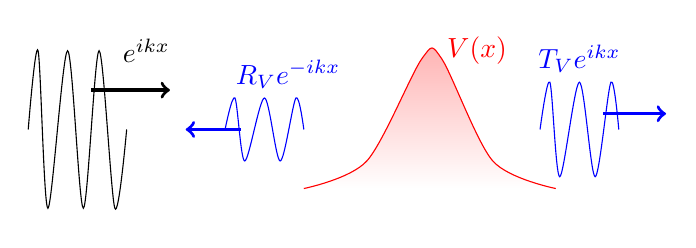
\begin{tikzpicture}
	\usetikzlibrary{fadings}
	
	\draw [->, very thick] (4.3,0.5) -- (5.3,0.5) ;
	\draw [->, very thick, blue] (6.2,0) -- (5.5,0) ;
	\draw [->, very thick, blue] (10.8,0.2) -- (11.6,0.2) ;
	\node at (5,1) {$e^{ikx}$};
	\node [blue] at (6.8,0.7) {$R_Ve^{-ikx}$};
	\node [blue] at (10.5,0.9) {$T_Ve^{ikx}$};
	\node [red] at (9.2,1) {$V(x)$};
	\draw [black] plot [smooth] coordinates {(3.5,0)  (3.625,1) (3.75,-1) (4,1) (4.2,-1) (4.4,1) (4.6,-1) (4.75,0)};
	
	\draw [blue] plot [smooth] coordinates {(6,0)  (6.125,0.4) (6.25,-0.4) (6.5,0.4) (6.7,-0.4) (6.9,0.4) (7,0)};
	\shade[top color=red!30,bottom color=white, draw=red] plot [smooth] coordinates {(7,-0.75) (7.8,-0.4) (8.5,0.9) (8.75,0.9) (9.4,-0.4) (10.2,-0.75)};
	
	\draw [blue] plot [smooth] coordinates {(10,0)  (10.125,0.6) (10.25,-0.6) (10.5,0.6) (10.7,-0.6) (10.9,0.6) (11,0)};
	\end{tikzpicture}
	\label{fig:asymptotics}
	\caption{Sketch of a scattering process of a plane wave with momentum $k$ into a potential $V(x)$ resulting into reflected and transmitted waves as Eq. (\ref{eq:asymptotics})}
\end{figure}
 At this point, we shall recall a few results of scattering theory. A deeper and more exhaustive analysis of the mathematical aspects of scattering theory could be found in [\citealp{scattering}].
\begin{lem}
	\label{lem:ex_of_sol}
	Let $V\in L^{1+}(\mR)$. Then the M\o{}ller operator $\Omega_V$ exists. Furthermore, the solution $x\mapsto\varphi_k(x)$ ($k>0$) of (\ref{eq:stationary_eq}) with the asymptotic conditions (\ref{eq:asymptotics}) exists and it is unique. In addition, for any $\hat{\psi}\in C_0^\infty(\mR)$,
	\begin{equation}
		(\Omega_VE_+\psi)(x)=\frac{1}{\sqrt{2\pi}}\int_{0}^{\infty}\nspace\!\varphi_k(x)\hat{\psi}(k)\, \dd k.
		\label{eq:asymptotic_sol}
	\end{equation}
\end{lem}

We will stick to report the references where finding an exhaustive proof of this lemma. Existence and uniqueness of solution $\varphi_k$ are a consequence of [\citealp[Chap. 5, Lemma 1.1]{scattering}]. Existence of $\Omega_V$, under milder assumptions on $V$, can be found in [\citealp[Chap. 5, Theorem 1.12]{scattering}].\\
\begin{oss}
	Let us dwell further on the meaning of Eq. (\ref{eq:asymptotic_sol}). We are considering a smooth wave-function $\psi$ with momentum representation $\hat{\psi}\in C^\infty_0(\mR)$, though we are interested only in "right-moving" solutions. Then, we will not consider the function $\hat{\psi}(k)$ for $k<0$. Considering only the "right-moving" components of $\psi$ we can think of it as the sum of plane wave-functions $e^{ikx}\hat{\psi}(k)$ (parametrized in $k>0$) which scatter into the potential $V$ giving the solutions $\varphi_k$. The integral of all this scattered components will give the solution $\Omega_VE_+\psi$.%them as independent plane wave-functions $e^{ikx}\hat{\psi}(k)$ (parametrized in $k>0$) which scatter into the potential $V$ giving the solutions $\varphi_k$. In the end, we just sum up all the interacting components in order to find out the solution $\Omega_VE_+\psi$.
\end{oss}
\begin{rem}
	From here on, we will consider only wave-functions $\psi$ such that $\hat{\psi}\in C^\infty_0(\mR)$ as in Lemma \ref{lem:ex_of_sol} in order to have a well defined asymptotic current operator $E_+\Omega_V^*J(f)\Omega_VE_+$.
\end{rem}

\begin{oss}
	Using (\ref{eq:asymptotic_sol}), we are able to estimate the expectation values of the asymptotic current operator as follows
	\begin{equation}
	(\psi|E_+\Omega^*_VJ(f)\Omega_VE_+\psi)=\int_{-\infty}^{\infty}\nspace\!\dd x\,f(x)\int_{0}^{\infty}\nspace\!\dd p\,\int_{0}^{\infty}\nspace\!\dd q\, \hat{\psi}^*(p)K_V(p,q,x)\hat{\psi}(q),
	\label{eq:density_product}
	\end{equation}
	where $K_V$ is
	\begin{equation}
	K_V(p,q,x)=\frac{i}{4\pi}[\partial_x\varphi_p^*(x)\varphi_q(x)-\varphi_p^*(x)\partial_x\varphi_q(x)].
	\label{eq:K_V}
	\end{equation}
\end{oss}

Following [\citealp{gand}], the next step in our analysis is to establish bounds on the solution $\varphi_k$ and $K_V$ relating them to their spatial asymptotics. As in the previous lemma, we will not give any proof, but only pointing to relevant references.
\begin{lem}
	\label{lem:bounds}
	Let $V\in L^{1+}(\mR)$ and let $\varphi_k$, with $k>0$, be the solution of (\ref{eq:stationary_eq}) with the asymptotics (\ref{eq:asymptotics}). Let $K_V$ be as in (\ref{eq:K_V}). Then, there exist constants $c_V,c_V',c_V'',c_V'''>0$ such that for all $x\in\mR$ and $p,q,k>0$
	\begin{align}
	%\begin{equation}
	|\varphi_k(x)|&\le c_V(1+|x|), \label{eq:bounds_1}\\
	%\end{equation} 
	%\begin{equation}
	 |\varphi_k(x)e^{ikx}|&\le c_V'\frac{1+|x|}{1+k}, \label{eq:bounds_2}\\
	%\end{equation} 
	%\begin{equation}
	 |\partial_x\varphi_k(x)-ik\varphi_k(x)|&\le c_V''\frac{1}{1+k}, \label{eq:bounds_3}\\
	%\end{equation} 
	%\begin{multline}
	 \left|K_V(p,q,x)-\frac{p+q}{4\pi}\varphi_p^*(x)\varphi_q(x)\right|&\le c_V'''(1+|x|). \label{eq:bounds_4}
	\end{align}
\end{lem}
The first two bounds in (\ref{eq:bounds_1}) and (\ref{eq:bounds_2}) can be deduced from [\citealp[Sec. 2, Lemma 1]{deift}], paying attention to the fact that the function $m(x,k)$ there corresponds to our $\varphi_k(x)e^{-ikx}/T_V(k)$, while $T_V(k)$ is such that $|T_V(k)|\le1$ and $T_V(k)=1+O(1/k)$ for large $k$ [\citealp[Sec. 2, Theorem 1]{deift}]. The last two bounds in (\ref{eq:bounds_3}) and (\ref{eq:bounds_4}), are consequence of (\ref{eq:bounds_1}) and (\ref{eq:bounds_2}). The constants $c_V,c_V',c_V'',$ and $c_V'''$ can be deduced from [\citealp{deift}] as functions of $V$, although they are not optimal and we will not use them during the following discussion.\\
With this information in mind, we have arrived to the first main result for backflow in scattering theory. We will prove the unboundedness of the asymptotic current operator $E_+\Omega_V^*J(f)\Omega_VE_+$ and the existence of backflow as well as the presence of negative parts of the spectrum, generalizing the results of the free situation, see Th. \ref{th:ex_averaged_backflow}.
\begin{theorem}[\textbf{Existence of backflow in scattering situations}]
	\label{th:ex_scat_back}
	Let $V\in L^{1+}(\mR)$. Then,
	\begin{itemize}
		\item[(a)] for every $f\in\mathcal{S}(\mR)$ with $f>0$, there is no finite upper bound on the asymptotic current operator $E_+\Omega_V^*J(f)\Omega_VE_+$,
		\item[(b)] for every $x\in\mR$, there is a sequence of normalized right-movers $\psi_n=E_+\psi_n$ such that $\lim_{n\to\infty}(\psi_n|\Omega_V^*J(x)\Omega_V\psi_n)=-\infty$.
	\end{itemize}
\end{theorem}
\begin{oss}
	Before proving Theorem \ref{th:ex_scat_back}, let us note that point (b) means that the backflow constant $\beta_V(f)$ could be negative for some positive $f$. Thus, averaged backflow exists in all scattering situations. The difference with the free case is that $\beta_0(f)$ ought to be negative for all positive Schwarz functions $f$, see Th. \ref{th:ex_scat_back} In scattering scenarios, we are not able to give an analogous statement for $\beta_V(f)$.
\end{oss}

\begin{proof}[Proof of Theorem \ref{th:ex_scat_back}]
	(a). To prove unboundedness of $E_+\Omega_V^*J(f)\Omega_VE_+$, we recall what done in Theorem \ref{th:ex_averaged_backflow} (b). Hence, we consider a right-mover $\psi=E_+\psi$ such that $\hat{\psi}\in C^\infty_0(\mR_+)$ and shift it to higher momenta defining the sequence $\hat{\psi}_n(p):=\hat{\psi}(p-n)$. In view of the unboundedness of $(\psi_n|E_+J(f)E_+\psi_n)$ from above [as in Theorem \ref{th:ex_averaged_backflow}(b)], we only need to show that the sequence $(\psi_n|(\Omega_V^*J(f)\Omega_V-J(f))\psi_n)$ is bounded as $n\to\infty$. In fact, from (\ref{eq:density_product}) it holds
	\begin{multline}
		(\psi_n|(\Omega_V^*J(f)\Omega_V-J(f))\psi_n)=\int_{-\infty}^{\infty}\nspace\! \dd x\, f(x)\int_{\mR_+^2}\dd p\,\dd q\,\times\\
		 \times\bigg\{\hat{\psi}^*_n(p)\hat{\psi}_n(q)\left[K_V(p,q,x)-\frac{p+q}{4\pi}\varphi_p^*(x)\varphi_q(x)\right]+\\
		 +\hat{\psi}^*(p)\hat{\psi}(q)\frac{p+q+2n}{4\pi}\left[\varphi_{p+n}^*(x)\varphi_{q+n}(x)-e^{i(q-p)x}\right]\bigg\},
	\end{multline}
	where $\varphi$ are the solutions taken from Lemma \ref{lem:ex_of_sol}. Since the norms $\|\hat{\psi}_n\|_{L^1}$ are independent from $n$, the first integrand is bounded in view of (\ref{eq:bounds_4}). (\ref{eq:bounds_1}) and (\ref{eq:bounds_2}) yield the same for the second integrand. This proves point (a).\\
	(b) Non-positivity of the asymptotic current operator $E_+\Omega_V^*J(f)\Omega_VE_+$ could be proved similarly. Here we take a sequence of right-movers $\psi_n^-$  as in Proposition \ref{prop:unboundedness}. Then, it suffices to show that $(\psi_n|(\Omega_V^*J(f)\Omega_V-J(x))\psi_n)$ is bounded in the same way as in point (a), using a suitable choice of $\chi$, such that $\hat{\chi}\in C^\infty_0(\mR_+)$) as in Proposition \ref{prop:unboundedness}.
\end{proof}

Now, we are ready for the main result of this chapter: the boundedness of the backflow constant $\beta_V(f)$ for every fixed non-negative $f\in\mathcal{S}(\mR)$, with potential $V\in L^{1+}(\mR)$. For this purpose, we need to take the asymptotic current operator $E_+\Omega_V^*J(f)\Omega_VE_+$ and split it into several terms (see in Observation (\ref{oss:split})).
\begin{oss}
	\label{oss:T_V}
	Consider the projector into the "left-movers" space $E_-$ from Definition \ref{def:projector_E+} and let the operator $T_V$ act by multiplication with the transmission coefficient $T_v(k)$ from (\ref{eq:asymptotics}) in momentum space. Hence, it holds true that
	\begin{itemize}
		\item[(i)]$T_V$ commutes with $E_\pm$ and $E_-T_VE_+=E_-E_+T_V=0$. The first statement descends from $E_\pm$ anf $T_V$ being defined as multiplicative operators in momentum space and the second from the identity $E_\pm E_\mp=0$.
		\item[(ii)]$E_-\Omega_VE_+=E_-(\Omega_V-T_V)E_+$ as consequence of point (i).
	\end{itemize}
\end{oss}

\begin{oss}[\textbf{Bounds of current operator}]
	\label{oss:split}
	Via the identities $E_-+E_+=\mathbb{I}$ and $(i+P)^{-1}(i+P)=\mathbb{I}$, it holds
	\begin{equation}
	\label{eq:split}
	\begin{aligned}
	E_+\Omega_V^*J(f)\Omega_VE_+&=E_+\Omega_V^*(E_-+E_+) J(f)(E_-+E_+)\Omega_VE_+\\
	& =E_+\Omega_V^*E_+ J(f)E_+\Omega_VE_+\\
	&+ E_+\Omega_V^*E_+J(f)(i+P)^{-1}E_-(i+P)(\Omega_V-T_V)E_+\\
	&+ E_+(\Omega_V^*-T_V^*)(-i+P)E_-(-i+P)^{-1}J(f)\Omega_VE_+.
	\end{aligned}
	\end{equation}
	Here we used the results from Observation \ref{oss:T_V}, the commutativity between $(i+P)$ and $E_\pm$ and $(i+P)^*=(-i+P)$. Note that the first term on the right side of (\ref{eq:split}) is bounded by the constant $\beta_0(f)$, as proved in Theorem \ref{th:ex_averaged_backflow}, and $\|E_+\|=\|\Omega_V\|=1$.\\
	We must evaluate the other terms on the right hand side of (\ref{eq:split}) in order to prove the existence of maximum backflow. In particular we want to show that
	\begin{equation}
	\begin{aligned}
	\inf(E_+\Omega_V^*J(f)\Omega_VE_+)&\ge \beta_0(f) -2\|J(f)(i+P)^{-1}\|\|(i+P)(\Omega_V-T_V)E_+\|\\ &\ge \beta_0(f)-2\|J(f)(i+P)^{-1}\|[2+\|P(\Omega_V-T_V)E_+\|],
	\end{aligned}
	\label{eq:split2}
	\end{equation}
	where the norms $\|J(f)(i+P)^{-1}\|$ and $\|P(\Omega_V-T_V)E_+\|$ ought to be finite.
\end{oss}

In order to estimate $\|J(f)(i+P)^{-1}\|$, it is useful to introduce the concept of Green's distribution. The Green distribution, or fundamental solution, of a linear differential operator $L$ is the distribution $G$ such that $LG=\delta$, where $\delta$ is the Dirac's delta distribution\footnote{see [\citealp[Chapt. 5, Sect. 3-4]{fried2}]}. In our case, we are interested in finding the Green's function of the time-independent Schr\"{o}dinger equation (\ref{eq:stationary_eq}).
\begin{prop}
	Consider the function $G_k(x)$ defined as 
	\begin{equation}
		G_k(x):=\frac{\sin(kx)}{k}\theta(x).
	\end{equation}
	Then, $G_k$ is the solution of equation $-G_k''(x)=k^2G_k(x)-\delta(x)$ in the sense of distributions, i.e. $G_k$ is the fundamental solution of the time-independent Schr\"{o}dinger equation (\ref{eq:stationary_eq}).
	\label{prop:green}
\end{prop}
The solution $\varphi_k$ of (\ref{eq:stationary_eq}) could be uniquely determined using $G_k$ via the following integral equation (Lippman-Schwinger equation) 
\begin{equation}
	\varphi_k(x)=T_V(k)e^{ikx}+\int_{-\infty}^{\infty}\nspace\! 2V(y)G_k(y-x)\varphi_k(y)\, \dd y,
	\label{eq:lippman}
\end{equation}
where (\ref{eq:lippman}) is the convolution between $G_k$ and $\varphi_k\cdot V$. With this information at hand,
\begin{prop}
	\label{prop:bound5}
	Let $V\in L^{1+}(\mR)$. Then
	\begin{equation}
		\|P(\Omega_V-T_V)E_+\|\le 2c_V\|V\|_{1+}\, ,
	\end{equation}
	with the constant $c_V$ being the one in Lemma \ref{lem:bounds}.
\end{prop}
\begin{proof}
	Consider $\xi,\psi$ such that $\hat{\xi},\hat{\psi}\in C_0^\infty(\mR)$ and $\psi=E_+\psi$. Lemma \ref{lem:ex_of_sol} yields
	\begin{equation}
	\begin{aligned}
	(\xi|P(\Omega_V-T_V)\psi)&=(P\xi|(\Omega_V-T_V)\psi)\\ &=\frac{i}{\sqrt{2\pi}}\int_{-\infty}^{\infty}\nspace\!\dd x\, {\xi'}^*(x)\int_{0}^{\infty}\nspace\! \dd k\, [\varphi_k(x)-T_V(k)e^{ikx}]\hat{\psi}(k).
	\end{aligned}
	\end{equation}
	The expression above may be rewritten in view of (\ref{eq:lippman}), using Fubini's theorem and integration by parts. Thus, we obtain
	\begin{equation}
	\label{eq:bound_5}
	\begin{aligned}
	(\xi|P(\Omega_V-T_V)\psi)&=\frac{i}{\sqrt{2\pi}}\int_{-\infty}^{\infty}\nspace \dd x\, {\xi'}^*(x)\int_{0}^{\infty}\nspace\!\dd k\,\int_{-\infty}^{\infty}\nspace\! \dd y\, 2V(y)G_k(y-x)\varphi_k(y).\\
	& = \frac{2i}{\sqrt{2\pi}}\int_{\mR^2}\nspace\!\dd x\,\dd y\int_{0}^{\infty}\nspace\!\dd k\, \xi(x)^*V(y)\cos[k(y-x)]\theta(y-x)\varphi_k(y)\hat{\psi}(k)
	\end{aligned}
	\end{equation}
	Consider the multiplicative operator $M_y$, with $y\in\mR$, defined as
	\begin{equation}
		(M_y\psi)(k):=\mathcal{F}^{-1}[\varphi_k(y)\hat{\psi}(k)]
	\end{equation}
	and the integral operator $I_y$
	\begin{equation}
		(I_y\hat{\psi})(x):=\theta(y-x)\int_{0}^{\infty}\nspace\!\cos[k(y-x)]\hat{\psi}(k)\, \dd k.
	\end{equation}
	As noted in [\citealp[Prop. 2]{gand}], %the last equation consists of a projection onto only the positive and even momentum part of $\psi$, a multiple of the Fourier transform, a multiplication by the Heaviside function, and a change of variables $x\mapsto y-x$. Thus,
	 $\|I_y\|\le\sqrt{2\pi}$ for all $y\in\mR$. Using Lemma \ref{lem:bounds} and (\ref{eq:bounds_1}), we establish the following bound for $M_y$:
	\begin{equation}
		\|M_y\psi\|\le (c_V(1+|y|))\|\psi\|\Rightarrow \|M_y\|\le c_V(1+|y|)\ \forall y\in\mR.
	\end{equation}
	Replacing the previous bounds in (\ref{eq:bound_5}), yields
	\begin{equation}
	\begin{aligned}
	|(\xi|P(\Omega_V-T_V)\psi)|&\le \frac{2\|\xi\|\|\psi\|}{\sqrt{2\pi}}\int_{-\infty}^{\infty}\nspace\!|V(y)|\|I_y\|\|M_y\|\,\dd y\\
	&\le 2c_V\|\xi\|\|\psi\|\int_{-\infty}^{\infty}\nspace\!|V(y)|(1+|y|)\,\dd y\\ &\le 2c_V\|V_y\|_{1+}\|\xi\|\|\psi\|.
	\end{aligned}
	\end{equation}
	Since $\xi$ and $\psi$ are taken respectively from a dense subspace of $L^2(\mR)$ and $E_+L^2(\mR)$, this concludes the proof.
\end{proof}

Summing up all results obtained in Observation \ref{oss:split}, (\ref{eq:split}), and Proposition \ref{prop:bound5}, it holds the following\footnote{see [\citealp[Th. 3]{gand}]}
\begin{theorem}[\textbf{Boundedness of backflow in scattering situations}]
	\label{th_backflow_scat}
	For any potential $V\in L^{1+}(\mR)$ and for any non-negative $f\in\mathcal{S}(\mR)$, there exists a lower bound on the spatially averaged backflow:
	\begin{equation}
		\beta_V(f)\ge\beta_0(f)-[2\|f\|_{\infty}+\|f'\|_{\infty}](2+2c_V\|V\|_{1+})>-\infty,
		\label{eq:backflow_scat}
	\end{equation}
	where $\|f\|_{\infty}:=\sup_{x\in\mR}|f(x)|$, $\beta_0(f)$ is the backflow constant in Th. \ref{th:ex_averaged_backflow}, and $c_V$ is the constant from Lemma \ref{lem:bounds}.
\end{theorem}
\begin{proof}
	To prove this bound we reconsider (\ref{eq:split2})
	\begin{equation}
		\inf(E_+\Omega_V^*J(f)\Omega_VE_+)\ge \beta_0(f)-2\|J(f)(i+P)^{-1}\|[2+\|P(\Omega_V-T_V)E_+\|].
		\label{eq:split3}
	\end{equation}
	Following Observation \ref{oss:split}, we must prove the existence of a bound for $\|P(\Omega_V-T_V)E_+\|$ and $\|J(f)(i+P)^{-1}\|$. The first one is given by Proposition \ref{prop:bound5}. To prove that for $\|J(f)(i+P)^{-1}\|$, we note from the definition of $J(f)$ in (\ref{eq:density_operator}) that
	\begin{equation}
		J(f)=\frac{1}{2}[Pf(X)+f(X)P]=\frac{1}{2}\bigg[[P,f(X)]+2f(X)P\bigg]=f(X)P-\frac{i}{2}f'(X).
	\end{equation}
	Hence we have $\|J(f)(i+P)^{-1}\|\le \|f\|_{\infty}+\frac{1}{2}\|f'\|_{\infty}$. Replacing everything in (\ref{eq:split3}), the thesis follows.
\end{proof} 

The last theorem concludes our investigation on the existence of backflow in an interacting scenario. We have shown that the asymptotic current operator $E_+\Omega_V^*J(f)\Omega_VE_+$ is bounded from below. Thus, in any scattering scenario backflow can occur, but its value spatially averaged under a non-negative test-function $f$ is always bigger than the constant $\beta_V(f)$. Note that \eqref{eq:backflow_scat} says very little about the actual value of this bound and a numerical analysis is needed for different types of potentials $V$. Some examples are given in [\citealp[Sect. IV]{gand}].